%************************************************
\chapter{Current mobile Platforms}\label{ch:m_plats}
%************************************************
Over the past few years competition between the different platform manufacturers has increased, leading to better products and features. In this chapter we will take a look at the most important players in mobile \ac{OS} race, in alphabetical order.

\begin{figure}[H]
    \begin{center}
        {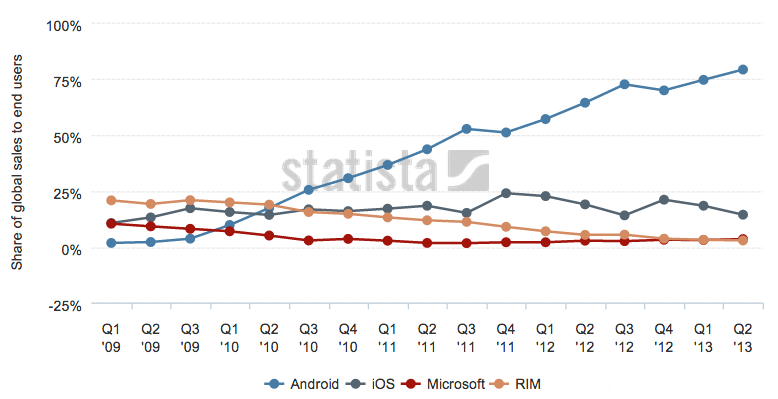
\includegraphics[width=1\linewidth]{gfx/statista-mobile}}
        \caption[Mobile OS share of global sales to end users]{Mobile OS share of global sales to end users\footnotemark}\label{fig:trend}
    \end{center}
\end{figure}
\footnotetext{Source: \url{http://www.statista.com/statistics/266136/global-market-share-held-by-smartphone-operating-systems}}\\

%***********************Ready
\section{Android}
\spacedlowsmallcaps{Android} is a Linux based \ac{OS} specially designed for touchscreen devices like smartphones or tablets. It began as the brain-child of a new company called Android, Inc. back in 2003. Since its inception, it has gained major popularity thanks to the plethora of devices that run it, giving users the option between low-budget and luxury phones and tablets. Its market share currently sits at over 75\% in terms of sales to end users.

Android, Inc. was founded in Palo Alto, California on October 2003 by Andy Rubin, Rich Miner, Nick Sears, and Chris White. Their goal was to develop smarter mobile devices that are more aware of its owner's location and preferences. They started developing an operating system for digital cameras, but once they realized the market wasn't big enough, they concentrated their efforts in producing an \ac{OS} for smartphones to rival Symbian and Windows Mobile.\cite{wikipedia:android}

Google bought Android, Inc. in 2005 and made it a wholly owned subsidiary. The most important employees stayed and started working on what later would become the Android Operating System.

Before Android's release, Google conducted meetings with many handset and chip manufacturers to discuss the creation of a new consortium, the Open Handset Alliance, with the goal to develop open standards for mobile devices. The Alliance was unveiled on November \nth{5}, 2007.\footnote{\url{http://www.openhandsetalliance.com/press_110507.html}}


After the first device with Android, the HTC Dream, was released on October 2008, there has been a major surge of devices using the operating system. Hardware manufacturers from all over the world have chosen Android as their favorite operating system, not only for smartphones and tablets but also for embedded devices like the Cotton Candy Stick\footnote{\url{http://www.fxitech.com/technology/for-android/}} from FXI Technologies and even for gaming consoles like the Ouya\footnote{\url{https://www.ouya.tv/discover/}}. %They have gone the Android route to give their devices a robust and secure operating system.


The development of system features and other components has been done at a steady pace, releasing new versions of the \ac{OS} every couple of months. The team has chosen to give colorful names to each release, always in alphabetical order and always named after a dessert or a sweet treat. A closer look at \autoref{fig:android1} and \autoref{fig:android2} should give you a better overview over the different versions of Android and what each of them brought forth.   

\begin{figure}[H]
    \hbox{
        \hspace{-4em}
        {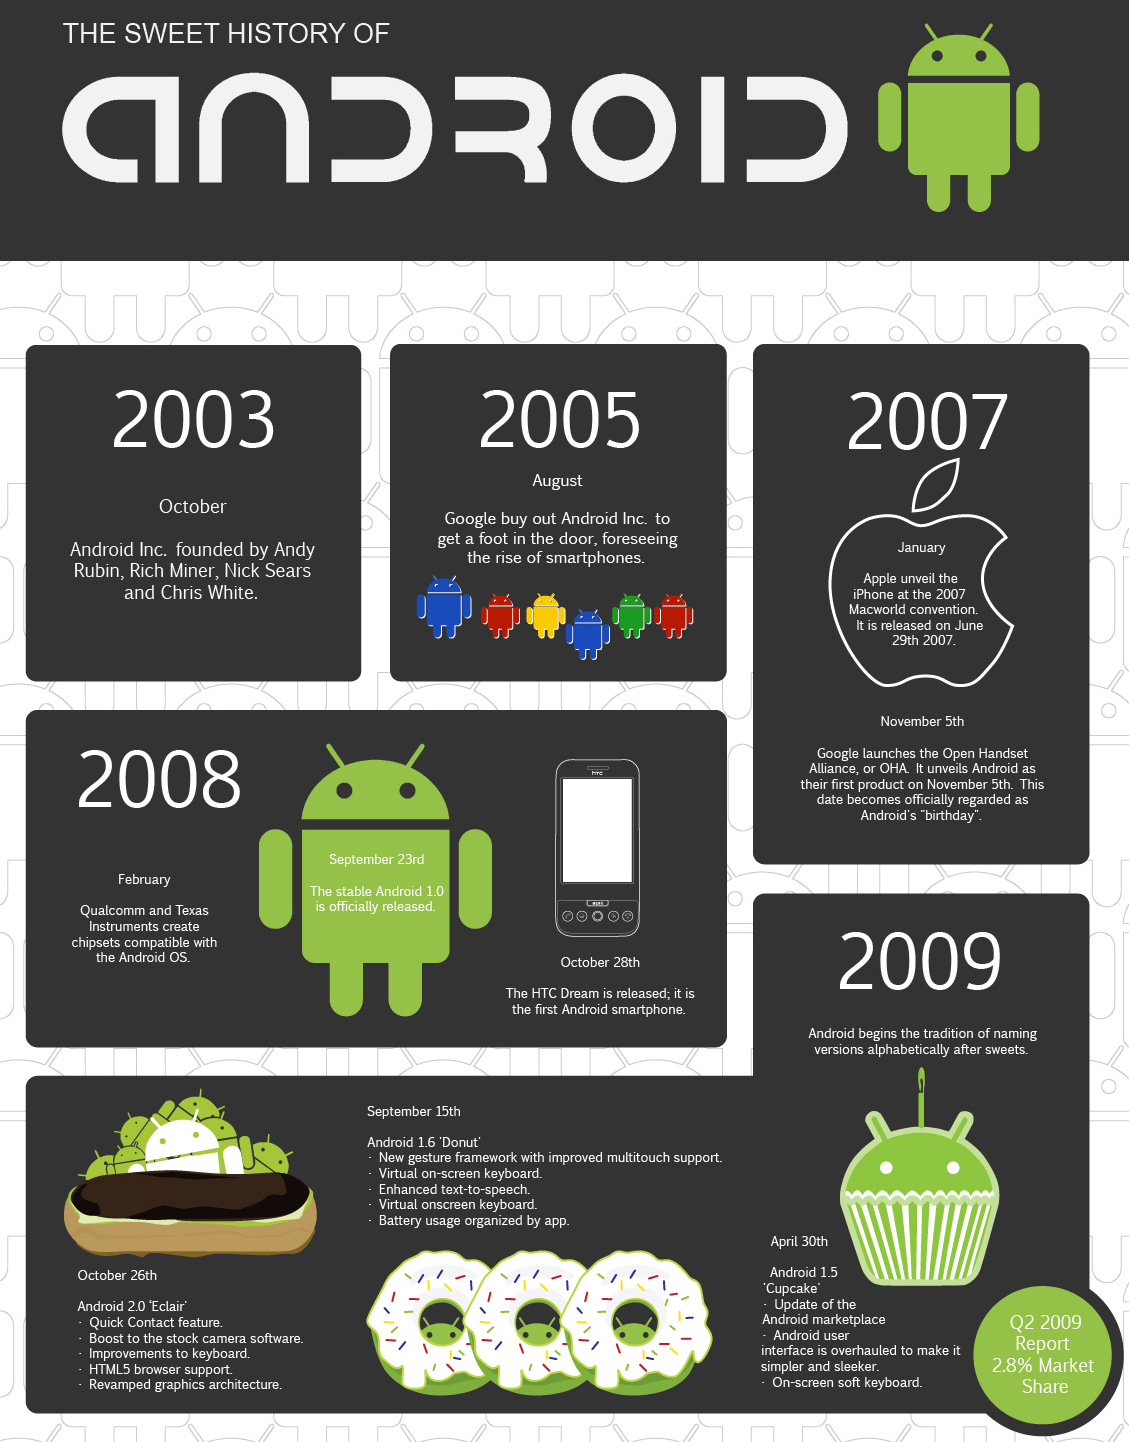
\includegraphics[width=1.5\linewidth]{gfx/android-history1}}
        \caption[Visual History of Android, Part 1]{Visual History of Android}\label{fig:android1}
    }
\end{figure}
\begin{figure}[H]
    \hbox{
        \hspace{-12em}
        {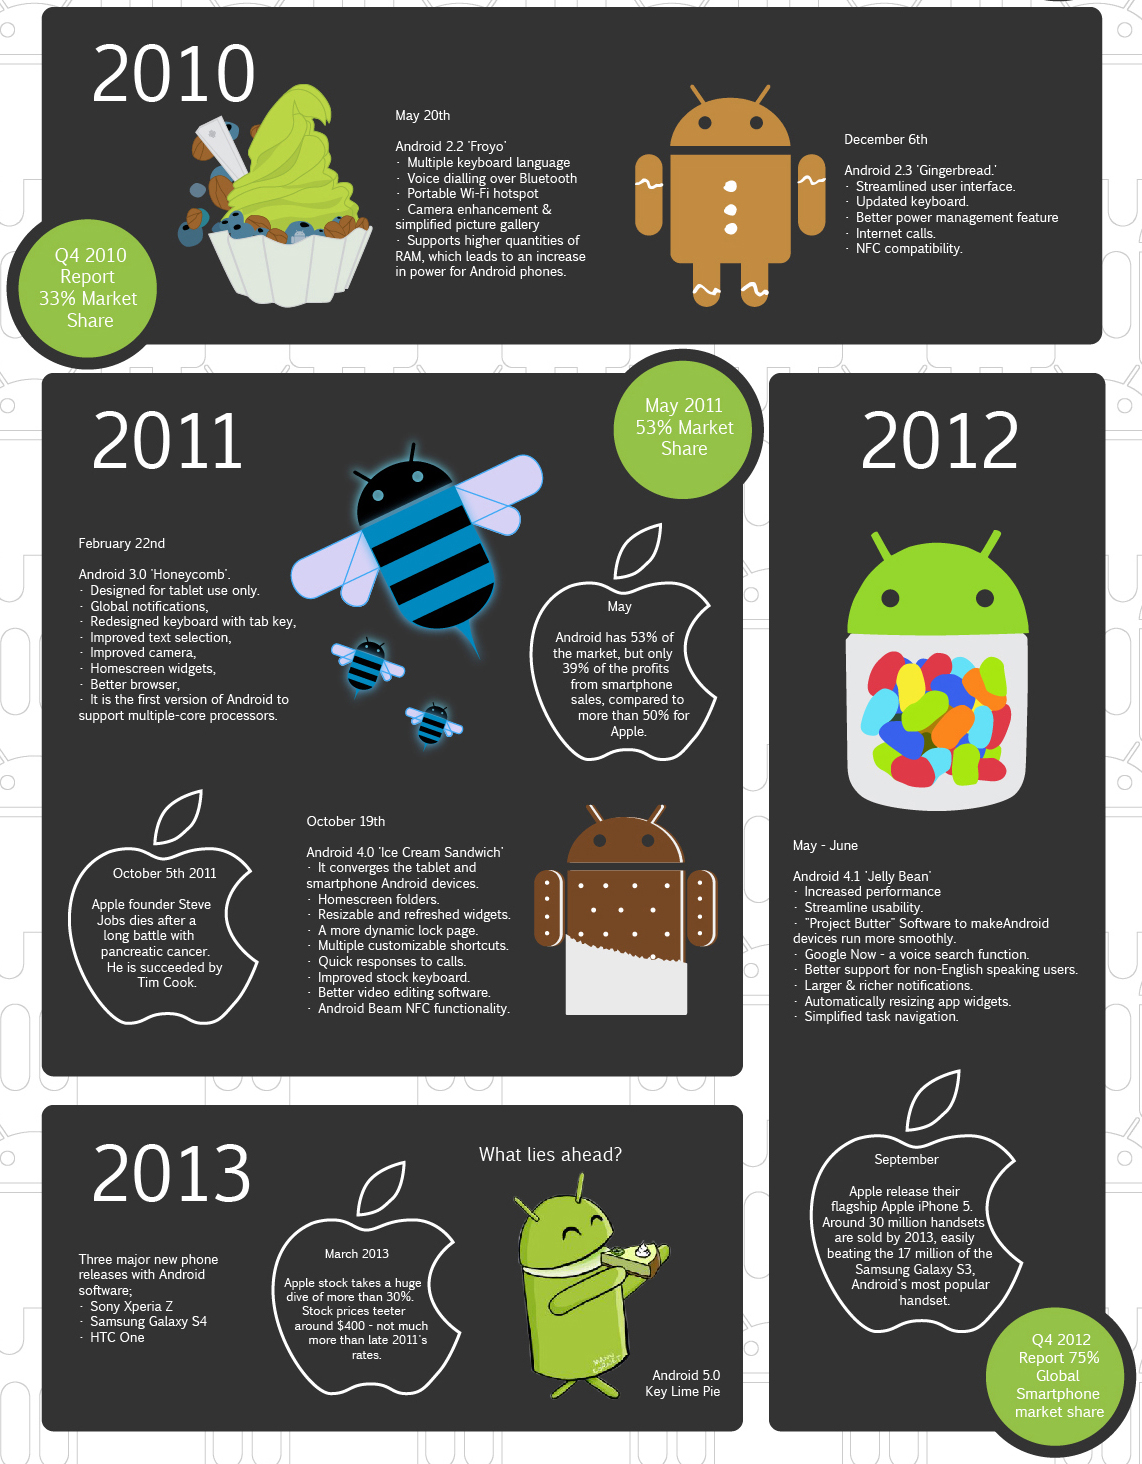
\includegraphics[width=1.55\linewidth]{gfx/android-history2}}
        \caption[Visual History of Android, Part 2]{Visual History of Android\footnotemark}\label{fig:android2}
    }
\end{figure}
\footnotetext{Source: \url{http://visual.ly/sweet-history-android}}\\

\subsection{The Android Open Source Project}
One of the best features and assets of Android is that the core operating system is 100\% Open Source. This allows anyone with the necessary knowledge to contribute to the development of the platform and also to modify it in every way they want.


This is exactly what the guys behind CyanogenMod\footnote{\url{http://www.cyanogenmod.org/}} have done. They took the regular Android Operating System and added many features and improvements to the core experience, making it the most popular unofficial Android \ac{OS}.\footnote{\url{http://lifehacker.com/5915793/most-popular-android-rom-cyanogenmod}}


But these types of modifications are not only common inside hobbyist communities. Big corporations also contribute code to the Android Project.\footnote{\url{http://libresoft.es/node/198}} Some even modify the code so much, that it becomes almost unrecognizable. That is exactly what Amazon did. They took the Android \ac{OS} and heavily modified it in order to install it in their Kindle Fire family of tablets.


Using an Open Source Model also guarantees Android an independent future from Google. Even if Google stops supporting \marginpar{Note: Google is unlikely to stop supporting Android} Android, the community will pick up the pieces and continue with its development and will guarantee its longevity.

%************************** 
\section{BlackBerry}
The Blackberry \ac{OS} is a proprietary mobile operating system developed by BlackBerry Ltd\marginpar{BlackBerry Ltd was until recently known as RIM (Research In Motion)} exclusively for its line of BlackBerry devices.

Research in Motion (RIM) was officially founded on March 7th, 1984 by Mike Lazaridis and Doug Fregin. Their main goal was to commercialize Budgie, a system that wirelessly displayed information on a TV screen. This endeavor generated enough business to let RIM take on side projects, but the real kick start was the introduction of one of the earliest wireless data networks, Mobitex. Software deals to support it led to the 1993 launch of RIMGate, the precursor to the BlackBerry Enterprise Server.

An article written by Jon \citeauthor{fingas:2013} in January, 2013 and published by EndGadget tells us the story of RIM around their first years:

\begin{quotation}
For its first two decades, RIM often showed the traits of a scrappy startup. It had nothing to lose and was willing to turn its business model on a dime to stay afloat. More importantly, it also had a simple, overriding determination to spread wireless data to the masses, no matter how that would come to pass. That gave it a leg up over contemporary technology stalwarts like Apple, Microsoft and Palm, all of whom were at least slightly behind RIM in seeing the value of truly instant mobile communication.
\cite{fingas:2013}
\end{quotation}


RIM started the BlackBarry brand in March 2002 with the BackBerry 5800. Since then may improvements have been made to the operating system and the devices running it. The BlackBerry platform is perhaps best known for its native support for corporate email. This allows complete wireless activation and synchronization with Microsoft Exchange, Lotus Domino, or Novell GroupWise email, calendar, tasks, notes, and contacts, when used with BlackBerry Enterprise Server.
\cite{wikipedia:bb}

\begin{quotation}
In 2005, the 8700 series took the 7100's sleeker aesthetic to the high-end; for many, it was the first modern BlackBerry, where a polished design, phone features and a full keyboard were all in one device. Not that RIM could rest on its laurels. Nokia, Palm and others had thrown themselves wholeheartedly into smartphones, and Microsoft's launches of Pocket PC 2002 and Windows Mobile provided a start for smartphone makers that would eventually play important roles, like HTC.
\cite{fingas:2013}
\end{quotation}


BlackBerry was the King of Smartphones around 2008-2009, surpassing its competitors by quite some margin, specially in the enterprise sector\footnote{\url{http://bgr.com/2011/12/13/apple-and-google-dominate-smartphone-space-while-other-vendors-scramble/}}; but now it is fighting for its life, having lost over \$1 Billion in 2013, mainly due to the failure to sell their latest flagship device, the BlackBerry Z10, in the expected quantities.\footnote{\url{http://arstechnica.com/business/2013/09/true-to-its-recent-prediction-blackberry-lost-over-1-billion-last-quarter/}} It now hopes to recover by selling the company.\footnote{\url{http://arstechnica.com/business/2013/08/blackberry-announces-that-it-may-sell-the-company/}}


The BlackBerry \ac{OS} hasn't been very popular among developers, either. With the launch of iOS and Android and their easy to use \ac{SDK} most developers flocked to the other platforms, leaving BlackBerry a barren territory, so much so that a single company developed 47,000 of the 120,000 applications currently available for BlackBerry devices.\footnote{\url{http://arstechnica.com/gadgets/2013/08/one-developer-makes-over-47000-of-blackberry-10s-120000-apps/}} As expected, market share has steadily fallen, to the point where it now sits at just under 3\% of total sales to end users.
  

%**************
\section{iOS}
\spacedlowsmallcaps{iOS} is a Unix-based (BSD) mobile operating system designed by Apple exclusively for its mobile devices, the iPhone and the iPad. After its unveiling in 2007, adoption rates for iOS powered devices skyrocketed, leaving it with a healthy 17\% share of global sales to end users by the end 2009, almost as much as BlackBerry. Since then, demand for new iOS devices has maintained between 13\% and 24\%, always growing a little whenever a new iPhone is announced.

The operating system was unveiled with the iPhone at the Macworld Conference \& Expo on January 2007, and released in June of that year. Apple did not specify a separate name for the \ac{OS}, stating simply that the iPhone runs OS X. Initially, third-party applications were not supported. The reasoning behind this decision was that developers could build web applications that would behave like native applications on the iPhone.\footnote{\url{http://www.engadget.com/2007/06/11/apple-announces-third-party-software-details-for-iphone/}} 

They reverted that policy, however, announcing later that year that a native \ac{SDK} was under development and that they planned to put it in developers' hands in February, but it wasn't until March, 2008, that Apple released the first beta, along with a name for the operating system, iPhone \ac{OS}.

It wasn't until June 2010 and after the release of the iPod Touch, a device that's basically an iPhone without the phone, that Apple decided to rebrand its mobile operating system to iOS.\footnote{\url{http://en.wikipedia.org/wiki/IOS}}

The history of iOS has been very straight forward and a new version has been unveiled every year. Unlike Google, Apple doesn't use code-names for every version of iOS, they just carry their version number. You can take a look at \autoref{fig:ios} for a more detailed description of every iOS version released until now.  

\begin{figure}[H]
    \begin{center}
        {\includegraphics[width=.95\linewidth]{gfx/ios-history}}
        \caption[Visual History of iOS]{Visual History of iOS\footnotemark}\label{fig:ios}
    \end{center}
\end{figure}
\footnotetext{Source: \url{http://visual.ly/history-ios}}\\

\subsection{Jailbreaking}
The very strict guidelines and restrictions imposed by Apple on their mobile operating system have led to many developers and hackers to come up with ways to circumvent them and use their rightfully owned devices to their full potential. This method is called \emph{Jailbreaking}\footnote{\url{http://en.wikipedia.org/wiki/IOS_jailbreaking}} \marginpar{Jailbreak: In other words, release their devices from the fictional jail imposed by Apple.} and it gives users access to many features that are present in Android devices, but either Apple has decided to block them or they allow the service providers to block them. The most notorious example in this particular area is Internet Sharing. 


In the United States, for example, Verizon blocks access to a system setting that allows you to share the mobile internet access of the device with other wireless devices, unless you pay an extra fee.\footnote{\url{http://arstechnica.com/information-technology/2013/10/how-i-share-my-iphones-internet-connection-without-paying-verizon-extra/}} This feature can also be blocked on Android devices, but unlike Apple, Google does allow applications that let you share your internet access into its store. Apple just blocks them. The only way around it, is to jailbreak your device.

The reason I mention this topic here is that it has become a really important issue, specially surrounding user rights. There have been many lawsuits worldwide regarding the legality of jailbreaking, some countries consider it illegal, but thanks to the EFF\footnote{\url{https://www.eff.org/}}\marginpar{EFF: Electronic Frontier Foundation} it is legal to jailbreak your phone in United States since 2010.\footnote{\url{http://www.wired.com/threatlevel/2010/07/feds-ok-iphone-jailbreaking/}}      

%**************************
\section{Windows}
\spacedlowsmallcaps{Windows Phone} is a mobile operating system developed by Microsoft that is based on the Windows CE and Windows NT Kernels. It was formerly known as Windows Mobile and the latest version is Windows Phone 8. Windows Mobile Devices never became popular outside the enterprise market, thus its share of global sales never grew past the 10.2\% after 2009. 


Windows Phone is largely incompatible with Windows Mobile, but its roots come from it so it is important to take a look at its history.
\subsection{Windows Mobile}
Microsoft's work on handheld portable devices began with research projects in 1990, leading to the start of the Windows CE project two years later.

Most versions of Windows Mobile have a set of standard features, such as multitasking and the ability to navigate a file system similar to that of Windows 9x and Windows NT, with support for many of the same file types. Much like its desktop counterpart, it comes bundled with a set of applications to perform basic tasks, like Internet Explorer Mobile, Windows Media Player and Office Mobile.\footnote{\url{http://en.wikipedia.org/wiki/Windows_Mobile}}

Despite having huge success on Desktop Environments and being one of the first players in mobile computing, Microsoft never succeeded in truly conquering the smartphone market. It managed to control 42\% of new sales in 2007\footnote{\url{http://bgr.com/2011/12/13/apple-and-google-dominate-smartphone-space-while-other-vendors-scramble/}}, but its lack of foresight in recognizing Apple's iPhone as a true competitor\footnote{\url{http://arstechnica.com/information-technology/2007/04/ballmer-says-iphone-has-no-chance-to-gain-significant-market-share/}}, meant it would ultimately arrive late to a market already dominated by Android and iOS.


\subsection{Windows Phone}
Work on a major Windows Mobile update may have begun as early as 2004 under the codename \textit{Photon}, but work moved slowly and the project was ultimately cancelled. In 2008, Microsoft reorganized the Windows Mobile group and started work on a new mobile operating system. This was expected to be released in 2009 as Windows Phone, but because of countless delays, Microsoft was forced to quickly update Windows Mobile and delivered version 6.5.\footnote{\url{http://www.mobiletechworld.com/2009/09/24/steve-ballmer-wishes-windows-mobile-7-had-already-launched-but-they-screwed-up/}} 

\begin{quotation}
Windows Phone was developed quickly. One result was that the new \ac{OS} would not be compatible with Windows Mobile applications. Larry Lieberman, senior product manager for Microsoft's Mobile Developer Experience, told eWeek: "If we'd had more time and resources, we may have been able to do something in terms of backward compatibility." Lieberman said that Microsoft was attempting to look at the mobile phone market in a new way, with the end user in mind as well as the enterprise network. Terry Myerson, corporate VP of Windows Phone engineering, said, "With the move to capacitive touch screens, away from the stylus, and the moves to some of the hardware choices we made for the Windows Phone 7 experience, we had to break application compatibility with Windows Mobile 6.5."
\cite{wikipedia:windows_phone}
\end{quotation}

Windows Phone finally launched on October \nth{10}, 2010, bringing many new features and changes. The biggest one was a completely redesigned \ac{UI} called Metro\marginpar{The Metro UI Design also exists on Windows 8}, using tiles to organize content on screen.  

For the release of Windows Phone 7, Microsoft partnered with Dell, HTC, LG and Samsung as manufacturers and stayed partners with HTC and Samsung for the release of Windows Phone 8.\footnote{\url{http://en.wikipedia.org/wiki/List_of_Windows_Phone_7_devices}}


The latest version of Windows Phone also saw a huge partnership with Nokia that would eventually result in Microsoft buying the phone manufacturer for \$7.2 Billion.\footnote{\url{http://www.microsoft.com/en-us/news/press/2013/sep13/09-02announcementpr.aspx}} This decision is widely seen as a desperate move to save the Windows Phone brand by saving from bankruptcy the only manufacturer that was able to maintain and slightly increase Windows Phone's market share.\footnote{\url{http://www.valuewalk.com/2013/09/microsoft-bought-nokia-to-save-windows-phone/}}  
 






%**************************Ready
\section{Other platforms worth noting}
The platforms mentioned above are the most popular ones. Together they control around 95\% of the mobile market, however, there are companies like Mozilla and Canonical that want to enter the competition and bring forth completely new ideas on what a mobile operating system should be.

\subsection{Firefox OS}
\spacedlowsmallcaps{Firefox OS} is Mozilla's entry to the mobile market. It hopes to revolutionize the mobile ecosystem by proposing that all applications for the device be programmed using Web Technologies.

\begin{quotation}
On July 25, 2011, Dr. Andreas Gal, Director of Research at Mozilla Corporation, announced the "Boot to Gecko" Project (B2G) on the mozilla.dev.platform mailing list. The project proposal was to "pursue the goal of building a complete, standalone operating system for the open web" in order to "find the gaps that keep web developers from being able to build apps that are, in every way, the equals of native apps built for the iPhone, Android, and Windows Phone." The announcement identified these work areas: new web APIs to expose device and \ac{OS} capabilities such as telephone and camera, a privilege model to safely expose these to web pages, applications to prove these capabilities, and low-level code to boot on an Android-compatible device.
\cite{wikipedia:firefox}
\end{quotation}

In 2012 B2G was rebranded as Firefox OS in honor of the company's flagship product, the Firefox Web Browser.

Some preview units have been shipped to journalists and developers, in order to gain some traction, but the system has not come to production, yet. 

In February 2013, Mozilla announced plans for a global commercial roll-out of Firefox OS. At a press conference before the start of Mobile World Congress in Barcelona Mozilla announced that the first wave of Firefox OS devices will be available to consumers in Brazil, Colombia, Hungary, Mexico, Montenegro, Poland, Serbia, Spain and Venezuela and that LG Electronics, ZTE, Huawei and TCL Corporation have committed to making Firefox OS devices.\footnote{\url{http://www.bbc.co.uk/news/technology-21522713}}
 

\subsection{Ubuntu Phone}
\spacedlowsmallcaps{Ubuntu Phone} is Canonical's horse in the mobile race. With it, Canonical hopes to disturb the mobile market by offering a single operating system capable of being a Mobile \ac{OS} and a Desktop \ac{OS}. As Canonical's own website puts it, 

\begin{quotation}
High-end smartphones have a brain as powerful as ultra-light laptops. Ubuntu uniquely enables a new category of convergence device - phones that dock to become full PCs and thin clients; enabling enterprise IT departments to replace phones, thin clients and laptops with a single secure corporate device.\\

Operators targeting the enterprise market with LTE can now deliver a full laptop/phone solution, with Windows apps delivered over LTE from the corporate data center. And operators in emerging markets can deliver desktop applications to the converged device over LTE as a premium data service.\footnote{\url{http://www.ubuntu.com/phone/operators-and-oems}}
\end{quotation}


Ubuntu Phone is still in the early stages of development, but has already gained the backing of major \ac{OEM} and carriers around the world. Once it hits the market, it will become the next player to watch, doubtlessly bringing new ideas and features to the table.
 